\section{Experiments}
\label{Sec:exp}

As a generic feature extraction and fusion solution, our method can be combined with any ConvNets.
%
To verify the effectiveness of the proposed HF-FCN in the building extraction task, extensive experiments have been conducted on three remote sensing datasets. 
%
In this section, the experimental setups are described including details of datasets, training settings, and the evaluation criteria.


\subsection{Datasets}
We test our method on three datasets: Massachusetts dataset, Vaihingen dataset, and Potsdam dataset.
These three datasets differ from each other on the building style, density, data channels, and spacial resolution. 

\paragraph{Massachusetts dataset}
%
Massachusetts dataset consists of 151 aerial images of the Boston area which covers roughly 340 square kilometers.
The resolution of each image is $1500\times 1500$ with the spacial resolution of 1 meter per pixel.
The images are composed of red, green and blue channels.
This dataset is built by Mnih~\cite{IEEEexample:mnih2013machine} while the ground-truth is produced by Saito et al.~\cite{IEEEexample:saito2016multiple}.
%
The dataset is split into three parts, a training set of 137 images, a test set of 10 images and validation set of 4 images.
To train the network, we create a set of image tiles for training and validation by sliding a ${256\times256}$ window with 64 stride from right to left, top to bottom. The detailed description is shown in Table~\ref{table:dataset-composition}.

\paragraph{Vaihingen dataset}
%
Vaihingen dataset is captured over Vaihingen which is a relatively small village with many detached buildings and small multi story buildings in Germany.
This dataset contains 16 labeled images whose spacial resolution is 9cm per pixel.7
It consists of near infra-red, red, green, blue imagery with corresponding normalized digital surface models (nDSMs) and row DSMs. The dataset is divided into the training set, validation set, and test set, which have 11 images, 2 images, and 3 images respectively. 
%
The same crop operations are done as the Massachusetts dataset.

\paragraph{Potsdam dataset}
%
In the Potsdam dataset, there are 24 labeled images whose ground sampling distance is 5cm.
This dataset shows a typical historic city with large building blocks. In order to grasp the global information of the building, the spacial resolution of the original image is reduced from 6000$\times$6000 to 1500$\times$1500.
Each image in this dataset contains 5-channel information: red, green, yellow, DSM and nDSM.
We split the dataset into training, validation and test sets in a proportion of $7:2:1$.



Data augmentation including data rotation and mirror flipping is applied to each dataset, respectively.
%
\comments{
Due to the other methods using dataset ${a)}$ do not extend the dataset, so the predict results on the original and extensible dataset $a)$ are both presented to make a fair comparison.
%
Besides, the data quantity of dataset ${b)}$ and ${c)}$ is not enough to make a adequate training, so we used the extensible dataset as our training set directly.
}
The detailed compositions of the three datasets are listed in Table~\ref{table:dataset-composition}.
Fig.~\ref{fig:dataset_sample} shows some patch samples of the three datasets.
The characteristics and challenges of the three datasets are:
\begin{itemize}
 \item The Massachusetts dataset has crowed buildings, which causes great difficulties for the separation of buildings.
 \item There is an obvious shadow occlusion in the Vaihingen dataset which may lead to a wrong segmentation in the part of the shadowed rooftop.
 \item Large intra class differences and small inter class differences are presented in the Potsdam dataset. One building consists of several materials while the roads and buildings appear in very similar colors. 
\end{itemize}


\begin{figure}
%\setlength{\abovecaptionskip}{-0cm}
%\setlength{\belowcaptionskip}{-2cm} 
\centering
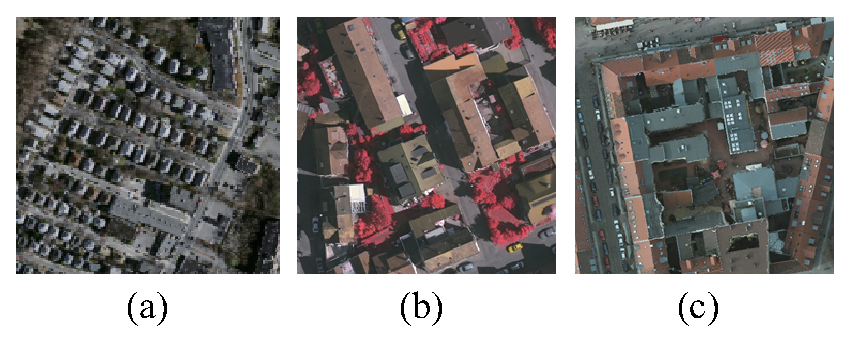
\includegraphics[width=8cm]{Figures/datasets.eps}
\caption{Sample patches on the three datasets. (a) Massachusetts dataset, (b) Vaihingen dataset, (c) Potsdam dataset.}
\label{fig:dataset_sample}
\end{figure}

\begin{table}
%\vspace{-0.2cm}
\setlength{\belowcaptionskip}{-2cm} 
 \centering
 \caption{Compositions of datasets}
 \label{table:dataset-composition}
 \begin{tabular}{c|ccc}
\hline
& Masschusetts & Vaihingen & Potsdam\\  \hline
Labeled images & 151& 16 &24\\ \hline
GSD & 1m & 9cm & 5cm\\ \hline
Bands & R,G,B & IR,R,G,DSM & IR,R,G,B,DSM\\ \hline
%Training set & \tabincell{c}{1,3,5,7,13,\\17,21,23,26,32,37} &\tabincell{c}{2\_10,3\_10,3\_11,3\_12,\\4\_11,4\_12,5\_10,5\_12,\\6\_8,6\_8,6\_10,6\_11,\\6\_12,7\_7,7\_9,7\_11,7\_12}\\ \hline
Training images &137 & 11 & 17\\ \hline
Training patches&75938 &115088 &85000\\ \hline
Training patch size& 256$\times$256 & 256$\times$256 & 256$\times$256\\ \hline
Validation images & 4 & 3 & 4\\ \hline
validation patches &2500 & 28376 &25000 \\\hline
Validation patch size & 256$\times$256 & 256$\times$256 & 256$\times$256\\ \hline
%Test set & 15,30 &2\_12,6\_7,7\_8 \\ \hline
Test images & 10 & 2 & 3\\ \hline
\end{tabular}
\end {table}



\subsection{Training Settings}
We first train the proposed HF-FCN on the Massachusetts dataset due to its large amounts of training data. The pre-trained model of VGG16 Net and ResNet \cxj{on which dataset? ImageNet?} are used to finetune our HF-FCN. 
%
We use the stochastic gradient descent algorithm with the learning rate divided by 10 for each 8000 iterations to train our network. 
%
The drop-out ratio is set to 0.5.
% 
When the HF-FCN converges on the dataset ${a)}$, we transfer it to the other datasets. \cxj{What do you mean by transfer? Fine-tuning? The input data has different number of channels.}
%
All experiments in this paper are conducted using Caffe and trained on a single NVIDIA Titan 12GB GPU. 
The hyper-parameters for each dataset are listed in Table~\ref{table:Train-Parameter}.

\begin{table}
%\vspace{-0.2cm}
%\setlength{\belowcaptionskip}{-2cm} 
\centering
\caption {Parameters for Network Training}
\label{table:Train-Parameter}
\begin{tabular}{c|c|c|c}
\hline
&Massachusetts &Vaihigen &Potsdam\\  \hline
%input size & 256$\times$256 &256$\times$256 \\
mini-batch size & 18& 15 & 15 \\
initial learning rate & $10^{-5}$ & $10^{-6}$ & $10^{-5}$\\
test\_interval&1000 & 1000 &1000\\
%type &SGD &SGD &SGD\\
training iteration & 10000 & 10000& 10000\\
momentum & 0.9 & 0.9 & 0.9\\
clip\_gradients & 16000& 10000 & 10000\\
weight\_decay & 0.02& 0.005 & 0.005\\ \hline
\end{tabular}
\end{table}

\subsection{Evaluation Metrics}
Several evaluation metrics are adopted in our work. 
For the Massachusetts dataset, the most common metrics are precision and recall.
The standard ($\rho$=0) and relaxed ($\rho$=3) precision and recall scores are used to evaluate the prediction results. 
Here the relaxed precision means the predicted pixels are within $\rho$ pixels of a true pixel while the relaxed recall is the true pixels are within $\rho$ pixels of a predicted pixel. \cxj{Check how other paper explain this.}
Moreover, the time cost is used to measure the efficiency of our HF-FCN. 
%
For the Vaihingen and Potsdam datasets, besides of the correctness and completeness,
we use the $F_1$ score as an additional evaluation metric \cxj{for what reason?}.


\comments{
\begin{equation}
 {completeness} = \frac{TP}{TP+FN},
\end{equation}
\begin{equation}
{correctness} = \frac{TP}{TP+FP},
\end{equation}
}
\begin{equation}
{F_1}= 2\cdot\frac{precision\cdot recall}{precision + recall}.
\end{equation}
%where TP indicates the true positives, FP implies the false positive, TN means the true negatives and FN refers to the false negatives.
